\documentclass[12pt,english]{scrartcl}

\usepackage{amsmath,amssymb}
%\usepackage[amssymb]{SIunits}
\usepackage{babel}
\usepackage[latin1]{inputenc}
\usepackage{graphicx}
\usepackage{color}
\usepackage[font={color=blue},figurename=Fig.,labelfont={it}]{caption}

\title{KOGW-PM-KNP: Edge detection Answers - Gaussian filtering}

\begin{document}

\maketitle

Complete the tasks using python. Your answers should include the code you wrote and written answers to the questions with relevant output images.

\section*{Task 1. Gaussian filtering of an image}

\begin{enumerate}
 \item Using the given equation for a 2D Gaussian filter, plot the output of a filter-convolved image with an appropriate sigma $\sigma$ value.
 \item[]
 \centering
 $G(x,y) = \frac{1}{2\pi\sigma^2} e^{-\frac{x^2+y^2}{2\sigma^2}}$
 \item[]
 \raggedright
 \color{blue}
 Plotting the various blurred images (Input image/ Gaussian filter/  Gaussian-blurred output) [2]
 \begin{figure*}[htbp]
 \centering
 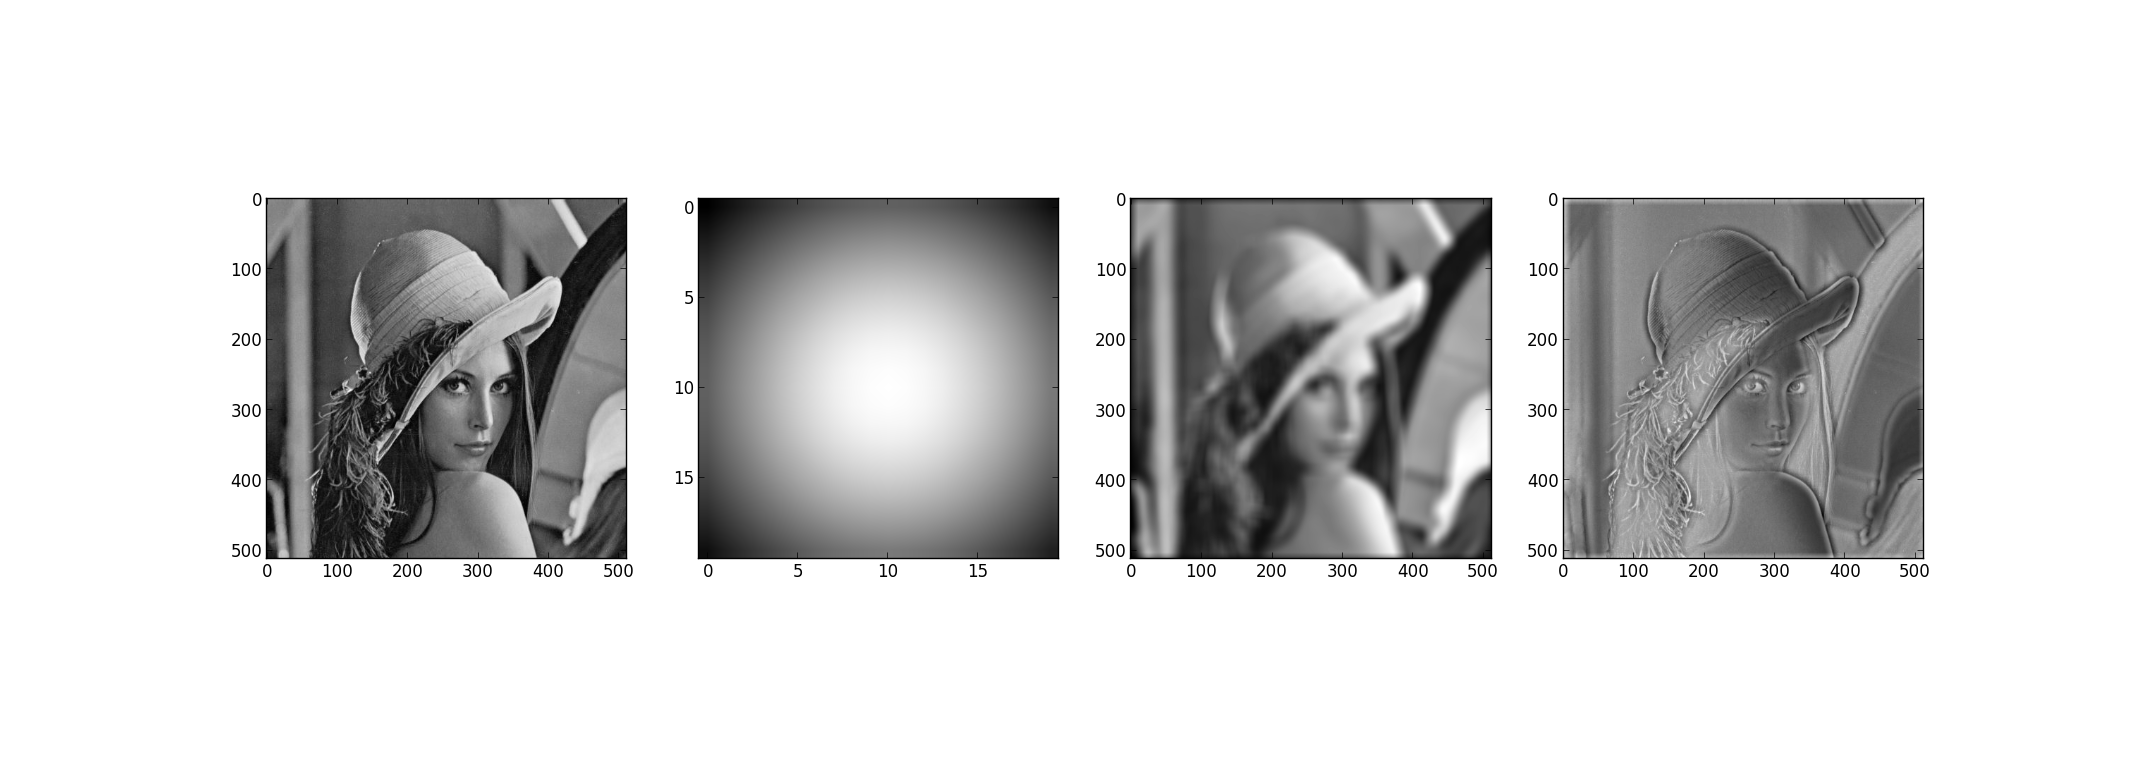
\includegraphics[width=1.0\textwidth]{/home/will/Documents/Git_Repository/Cog_Psy_Lectures/Cog_Psy_Lectures/Figures/Edge_detection_1/Figure1ED.png} 
 \caption{From left to right: Original image, Gaussian filter, Gaussian blurred image,  "edge-detected" output (for T.2)}
 \label{fig:lena_gauss}
 \end{figure*}

 
 \color{black} 
 \item What type of filter results from a high $\sigma$ value? 
 \color{blue}
 \item[]
 Low-pass filter [1]  
 
 \color{black}
 \item Can you think of a way of extracting high frequency components from an image using only a low frequency filtered image? Plot such an image and comment on its quality
 \item[]
 \color{blue}
 Subtract the low-pass filtered image from the original image. [1] \\
 \item[]
 Roughly an edge-detected image plotted, low quality (far-right Fig. 1). [1] \\
 \item[]
 \color{black}
 \item[] \textit{Hint: Use PIL.Image.open to import your image, and from scipy.signal use the convolve2d (with mode='same') function for the convolution.} \\
 \item[]

 \end{enumerate}

\section*{Task 2. Difference of Gaussian filtering of an image}

\begin{enumerate}
 \color{black}
 \item Create a Difference of Gaussian (DOG) filter by applying two different sigma valued Gaussian  filters to the original image and then subtracting the two outputs from each other. \\ 
 \color{blue}
 \item[]
 Produce a DOG filter and plot the output [2] \\

 \begin{figure*}[htbp]
 \centering
 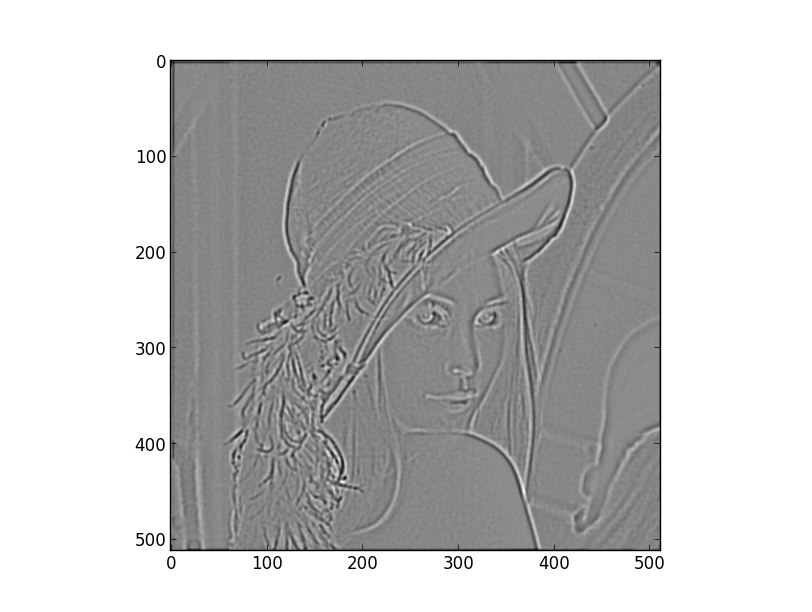
\includegraphics[width=0.3\textwidth]{/home/will/Documents/Git_Repository/Cog_Psy_Lectures/Cog_Psy_Lectures/Figures/Edge_detection_1/Figure2ED.png}
 \caption{Output of difference of Gaussian filtered image}
 \label{fig:lena_edge}
 \end{figure*}

 \color{black}
 \item Try to find optimum sigma values for detecting edges in an image.
 \color{blue}
 \item[]
 Optimum filter sizes have low sigma values e.g. 1 and 2. Must be different, low values.
 
 \color{black}
 \item Comment on differences between this filter and the first. \\
 \color{blue}
 Any 2 from below:
 \begin{itemize}
 \item Higher quality filter 
 \item Less image noise
 \item More easily controlled
 \end{itemize}
\end{enumerate}

\section*{Task 3. Phase and Fourier 1}

\section*{Task 4. Phase and Fourier 2}

 
\end{document}